\documentclass[a4paper, 12pt]{article}

%\usepackage{cmap}
\usepackage[T2A]{fontenc}
\usepackage[utf8]{inputenc}
\usepackage[english, russian]{babel}
\usepackage{graphicx}
\usepackage[top=1in, bottom=1in, left=3.2cm, right=2.6cm]{geometry}
\graphicspath{./}
\usepackage{biblatex}
\addbibresource{lib.bib}
\linespread{1.5}

\usepackage{listings}
\usepackage{color}
\usepackage{amsmath}

\begin{document}
	
\begin{titlepage}
	\fontsize{12pt}{12pt}\selectfont
	\begin{figure}[t!]
		\centering
		
\includegraphics[scale=0.8]{bmstu}
	\end{figure}
	
	\noindent\rule{15cm}{3pt}
	\newline\newline
	\noindent 
	ФАКУЛЬТЕТ 
	\underline{«Информатика и системы управления»} \newline\newline
	
	\noindent КАФЕДРА \underline{«Программное обеспечение ЭВМ и информационные технологии»}\newline\newline\newline\newline\newline\newline
	
	\centering {\LARGE Отчет по лабораторной работе № 7}
	\vspace{3mm}
	
	\centering {\LARGE По курсу "Анализ Алгоритмов"
		\vspace{10mm}	
		
		\centering \bf Поиск в словаре}
	\vspace{10mm}
	
	
	\begin{flushright}
		{\large	Студент:\\ Турсунов Жасурбек Рустамович \\ Группа: ИУ7-56Б
			\vspace{5mm}
			\\Преподователи: \\ Волкова Лилия Леонидовна \\ Строганов Юрий Владимирович}
	\end{flushright}
	
	\begin{center}
		\vfill
		Москва, \the\year
		~г.
	\end{center}
\end{titlepage}

\tableofcontents
\clearpage
\newpage

\section*{Введение}
\addcontentsline{toc}{section}{Введение}


	\hspace*{5mm}Целью данной лабораторной работы является изучение способа эффективного по времени и по памяти поиска по словарю.
	\\ \hspace*{5mm} Словарь, или ассоциативный массив, – абстрактный тип данных (интерфейс к хранилищу данных), позволяющий хранить пары вида «(ключ, значение)» и поддерживающий операции добавления пары, а также поиска
	и удаления пары по ключу.\cite{dict}
	\\ \hspace*{5mm}В паре ($k$, $v$) значение $v$ называется значением, ассоциированным с ключом $k$. Где $k$ – это $key$, a $v$ – $value$. Семантика и названия вышеупомянутых операций в разных реализациях ассоциативного массива могут отличаться.
	\\ \hspace*{5mm}Ассоциативный массив с точки зрения интерфейса удобно рассматривать как обычный массив, в котором в качестве индексов можно использовать не только целые числа, но и значения других типов – например, строки. 
	\newline \hspace*{5mm} В ходе лабораторной предстоит выполнить следующие задачи: 
	\begin{enumerate}
		\item рассмотреть и изучить алгоритмы полного перебора, двоичного поиска и эффективного поиска по словарю;
		\item сравнить временные характеристики каждого из рассмотренных алгоритмов;
		\item на основе проделанной работы сделать выводы.
	\end{enumerate}
	
\clearpage
\newpage
\section{Аналитическая часть}
	\hspace*{5mm} В данной части будут представлены теоретические сведения о рассматриваемых алгоритмах.
	\subsection{Алгоритм полного перебора}
	\hspace*{5mm} Алгоритмом полного перебора называют метод решения задачи, при котором по очереди рассматриваются все возможные варианты исходного набора данных. В случае словарей будет произведен последовательный перебор элементов словаря до тех пор, пока не будет найден необходимый. Сложность такого алгоритма зависит от количества всех возможных решений, а время решения может стремиться к экспоненциальному времени работы.
	\\ \hspace*{5mm} Пусть алгоритм нашёл элемент на первом сравнении, тогда, в лучшем случае, будет затрачено $k_0+k_1$ операций, на втором – $k_0 + 2k_1$, на последнем – $k_0+Nk_1$. Тогда средняя трудоёмкость может быть рассчитана по формуле 1, где $\Omega$ – множество всех возможных случаев.
	\begin{multline}
		\sum\limits_{i\in\Omega} \rho_i \cdot f_i = (k_0 + k_1)\frac{1}{N + 1} + (k_0 + 2k_1)\frac{1}{N + 1} +  (k_0 + 3k_1)\frac{1}{N + 1} + (k_0 + Nk_1)\frac{1}{N + 1} +\\+ (k_0 + Nk_1)\frac{1}{N + 1} = 
		k_0\frac{N + 1}{N + 1} + k_1 + \frac{1 + 2 + \dots + N + N}{N + 1} = k_0 + k_1(\frac{N}{N + 1} + \frac{N}{2}) = \\ = k_0 + k_1(1 + \frac{N}{2} - \frac{1}{N + 1})
	\end{multline}
	\subsection{Алгоритм двоичного поиска}
	\hspace*{5mm} Алгоритм двоичного поиска применяется к заранее упорядоченному словарю.\cite{bin} Проесс двоичного поиска можно описать при помощи шагов:
	\begin{enumerate}
		\item получить значение ключа, находящееся в середине словаря, и сравнить его с данным;
		\item в случае, если значение меньше (в контексте типа данных) данного, продолжить поиск в левой части словаря, в обратном случае – в правой;
		\item на новом интервале получить значение ключа из середины этого интервала и сравнить его с данным;
		\item продолжать поиск до тех пор, пока найденное значение ключа не будет равно данному.
	\end{enumerate}
	\hspace*{5mm}Поиск в словаре с использованием данного алгоритма в худшем случае будет иметь трудоемкость $O(log_2N)$, что быстрее поиска при помощи алгоритма полного перебора. Но стоит учитывать тот факт, что данный
	алгоритм работает только для заранее упорядоченного словаря. В случае большого объема данных и обратного порядка сортировки может произойти так, что алгоритм полного перебора будет эффективнее по времени, чем
	алгоритм двоичного поиска.
	\subsection{Алгоритм частотного анализа}
	\hspace*{5mm}Алгоритм частотного анализа на вход получает словарь и на его основе составляется частотный анализ. Чтобы провести частотный анализ нужно взять первый элемент каждого значения в словаре по ключу и подсчитать частотную характеристику, т.е. сколько раз этот элемент встречается в качестве первого элемента. По полученным значениям словарь разбивается на сегменты так, что все элементы с одинаковым первым элементом оказываются в одном сегменте.
	\\ \hspace*{5mm} Сегменты упорядочиваются по значению частотной характеристики так, чтобы к элементы с наибольшей частотной характеристикой был самый быстрый доступ.
	\\ \hspace*{5mm} Далее каждый сегмент упорядочивается по значению. Это необходимо
	для реализации бинарного поиска, который обеспечит эффективный поиск
	в сегменте при сложности $O(log_2N)$.
	\\ \hspace*{5mm} Таким образом, сначала выбирается нужный сегмент, а затем в нем проводится бинарный поиск нужного элемента. Средняя трудоёмкость при длине алфавита $M$ может быть рассчитана по формуле 2.
	\begin{equation}
		\sum\limits_{i\in[1, M]}(f_{select} + f_{search}) + \rho_i
	\end{equation}
	\subsection{Описание словаря}
	\hspace*{5mm} Словарь, реализованный в данной работе, имеет вид ${id: number, email: string}$, что представляет собой базу данных о пользователях с их уникальной почтой.
	\subsection{Вывод}
	\hspace*{5mm} Были рассмотрены разные алгоритмы поиска в словаре. Дана предварительная оценка времени для каждого алгоритма.


\newpage
\section{Конструкторская часть}
	\hspace*{5mm} В данном разделе представлены схемы рассматриваемых алгоритмов.
	

	\subsection{Разработка алгоритмов}
	\hspace*{5mm} На рисунках 1, 2 и 3 приведены схемы алгоритмов поиска в словаре перебором, двоичным поиском и частотным анализом соответственно. 
	\begin{figure}[h]
		\centering 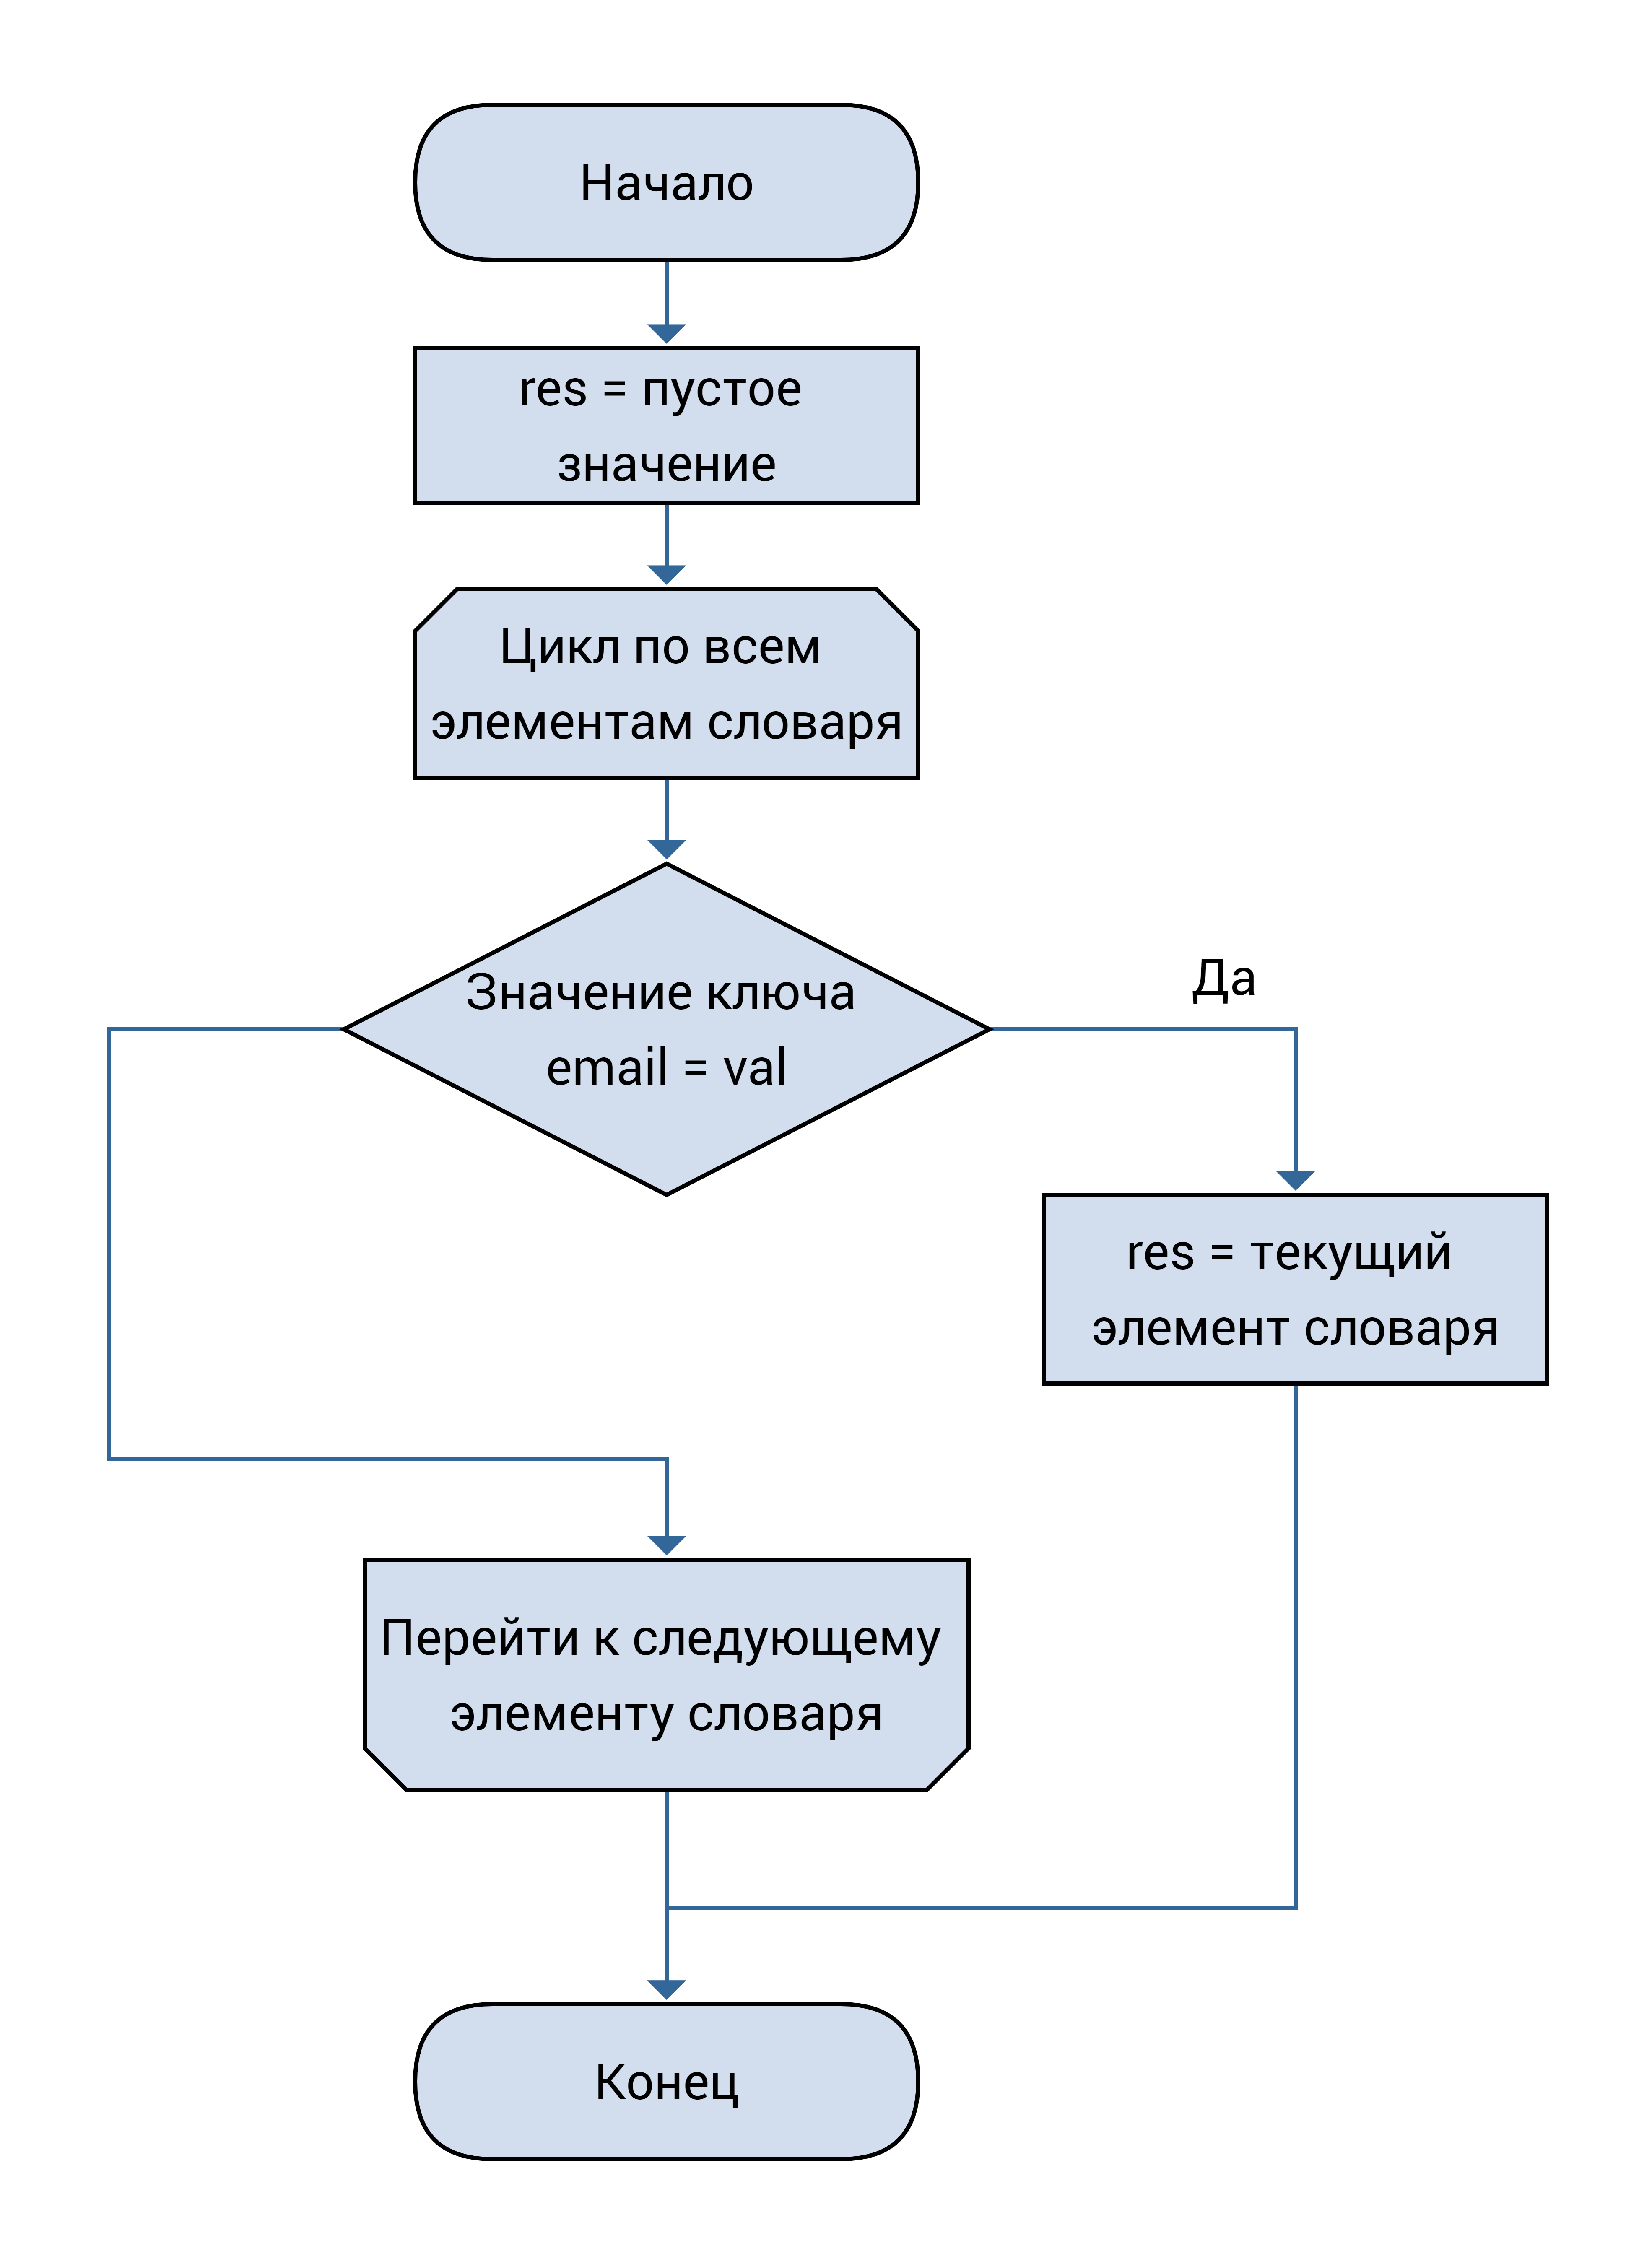
\includegraphics[scale=0.085]{full}
		\centering\caption{Схема алгоритма полного перебора в словаре.}
	\end{figure}
	\clearpage
	\newpage
	\begin{figure}[h!]
		\centering 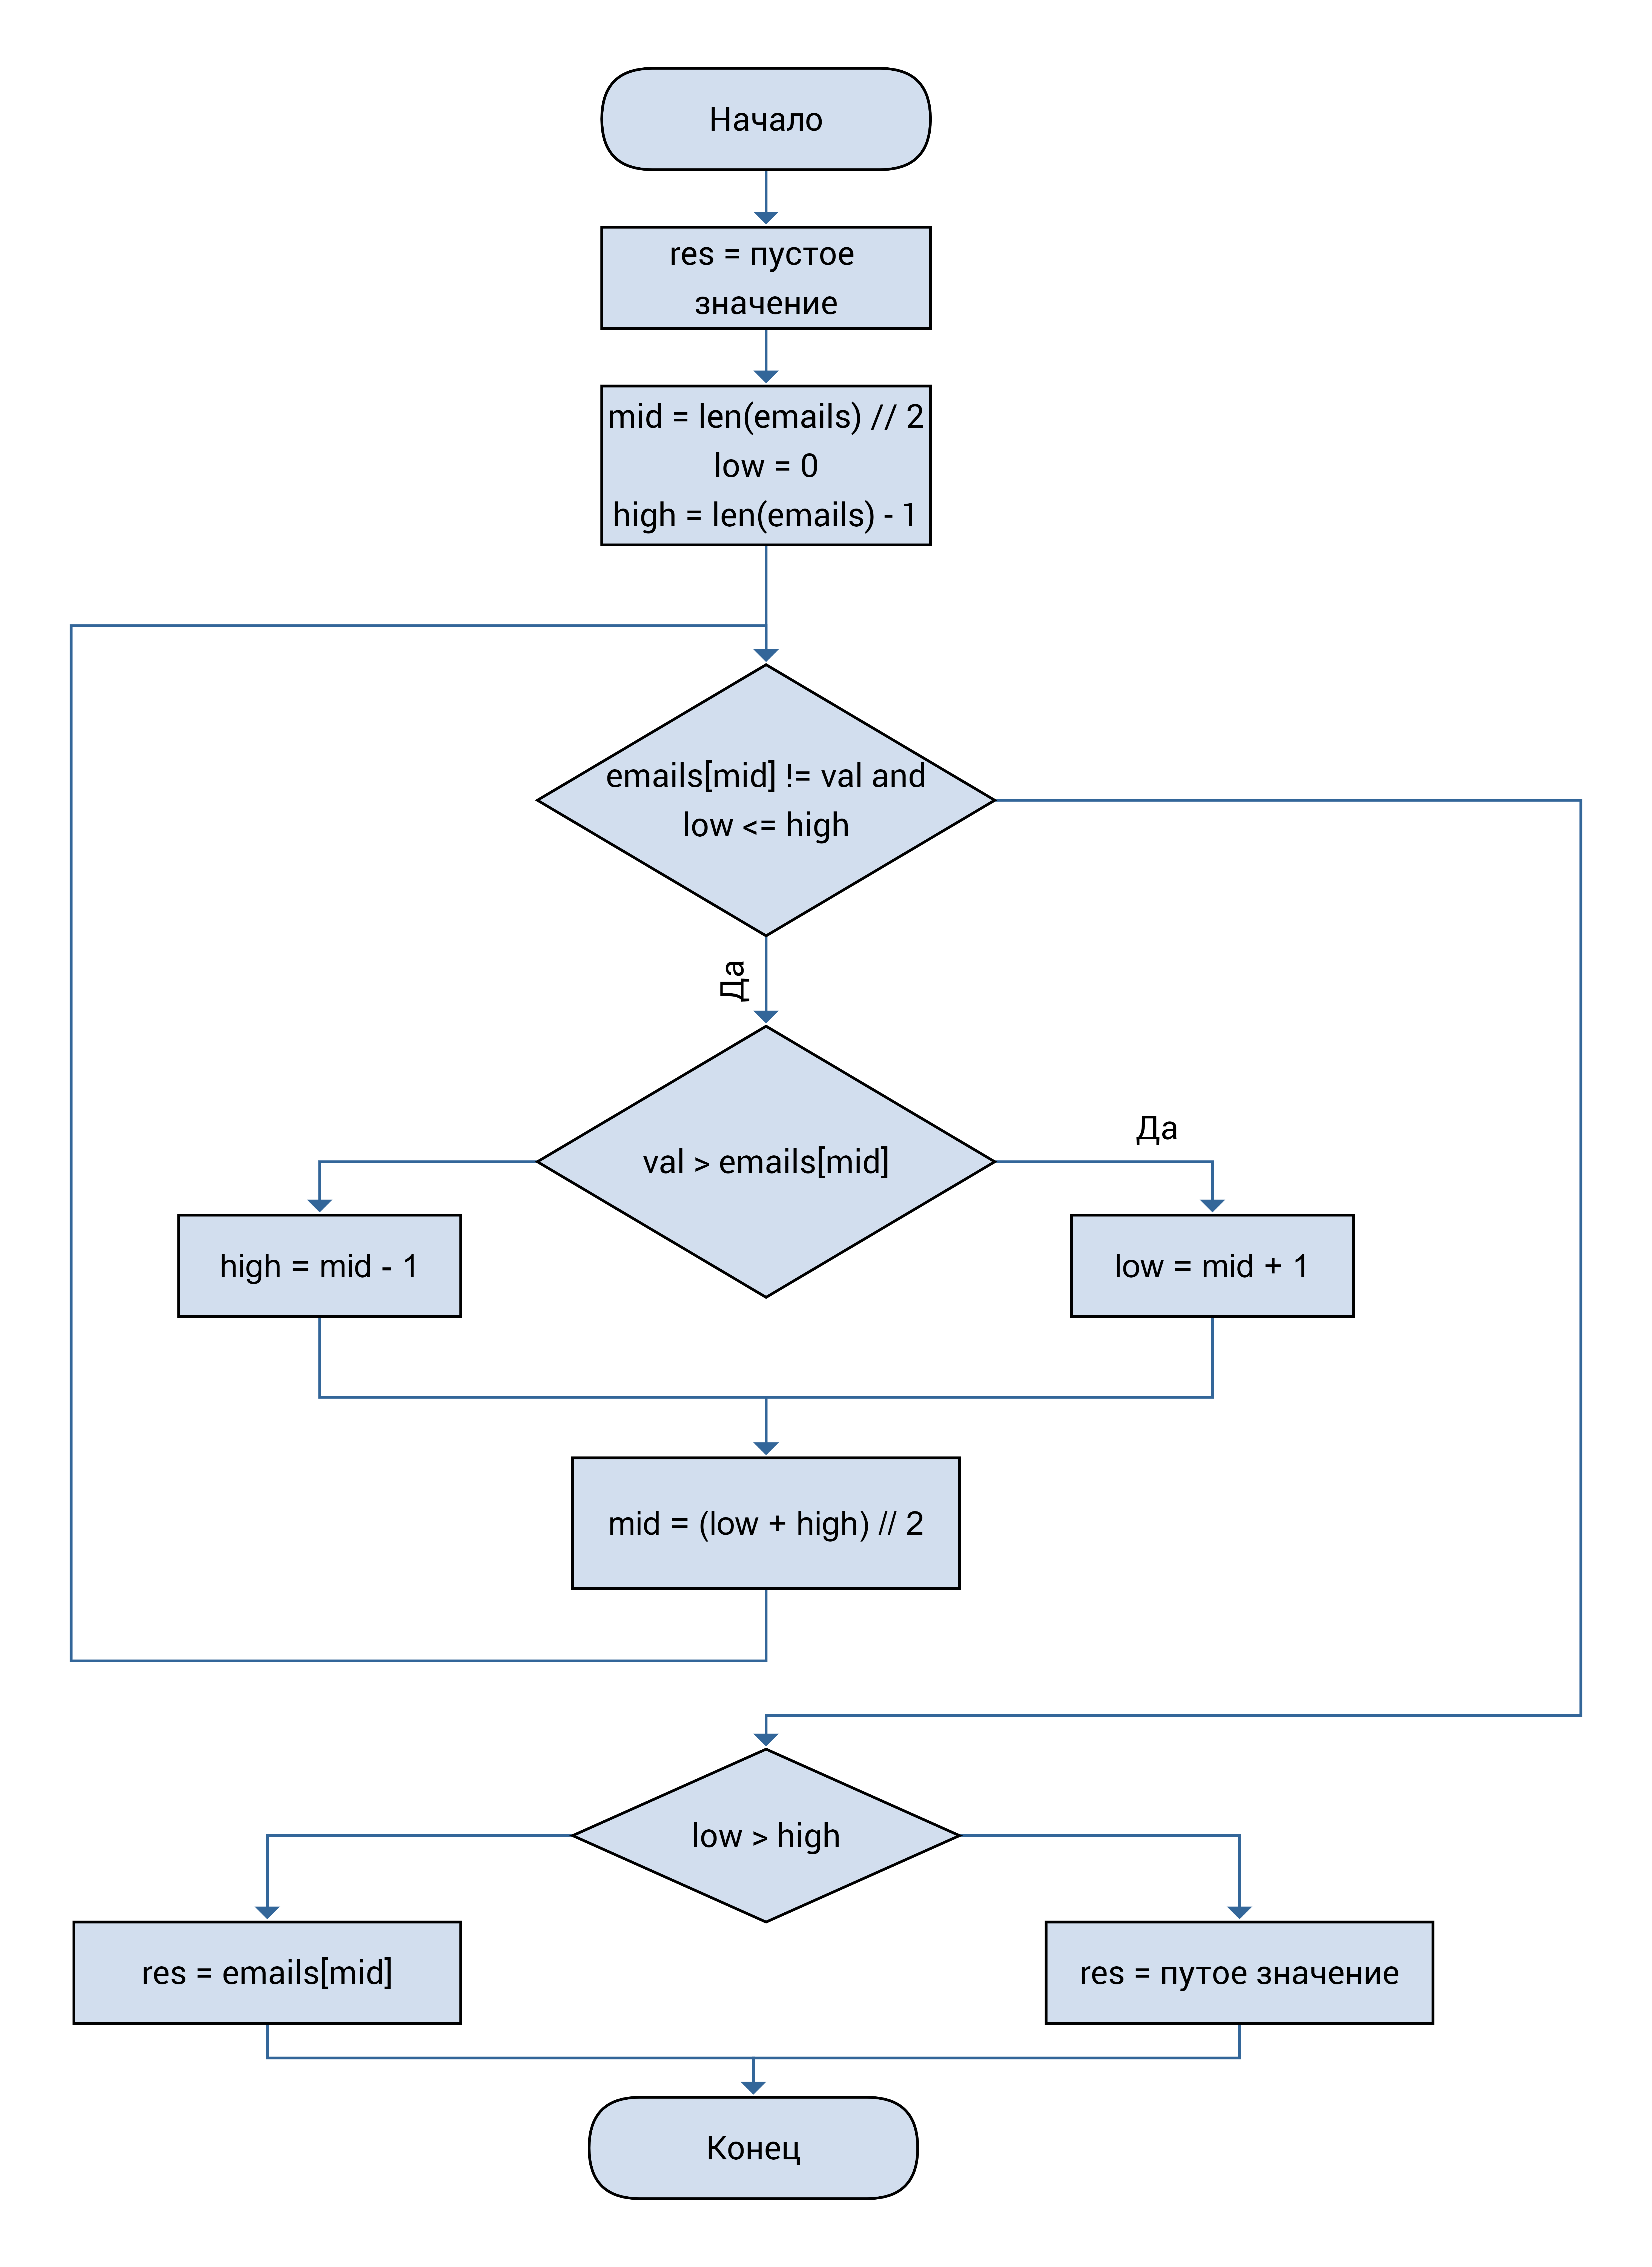
\includegraphics[scale=0.07]{bin}
		\centering\caption{Схема алгоритма бинарного поиска в словаре.}
	\end{figure}
	\clearpage
	\newpage
	\begin{figure}[h!]
		\centering 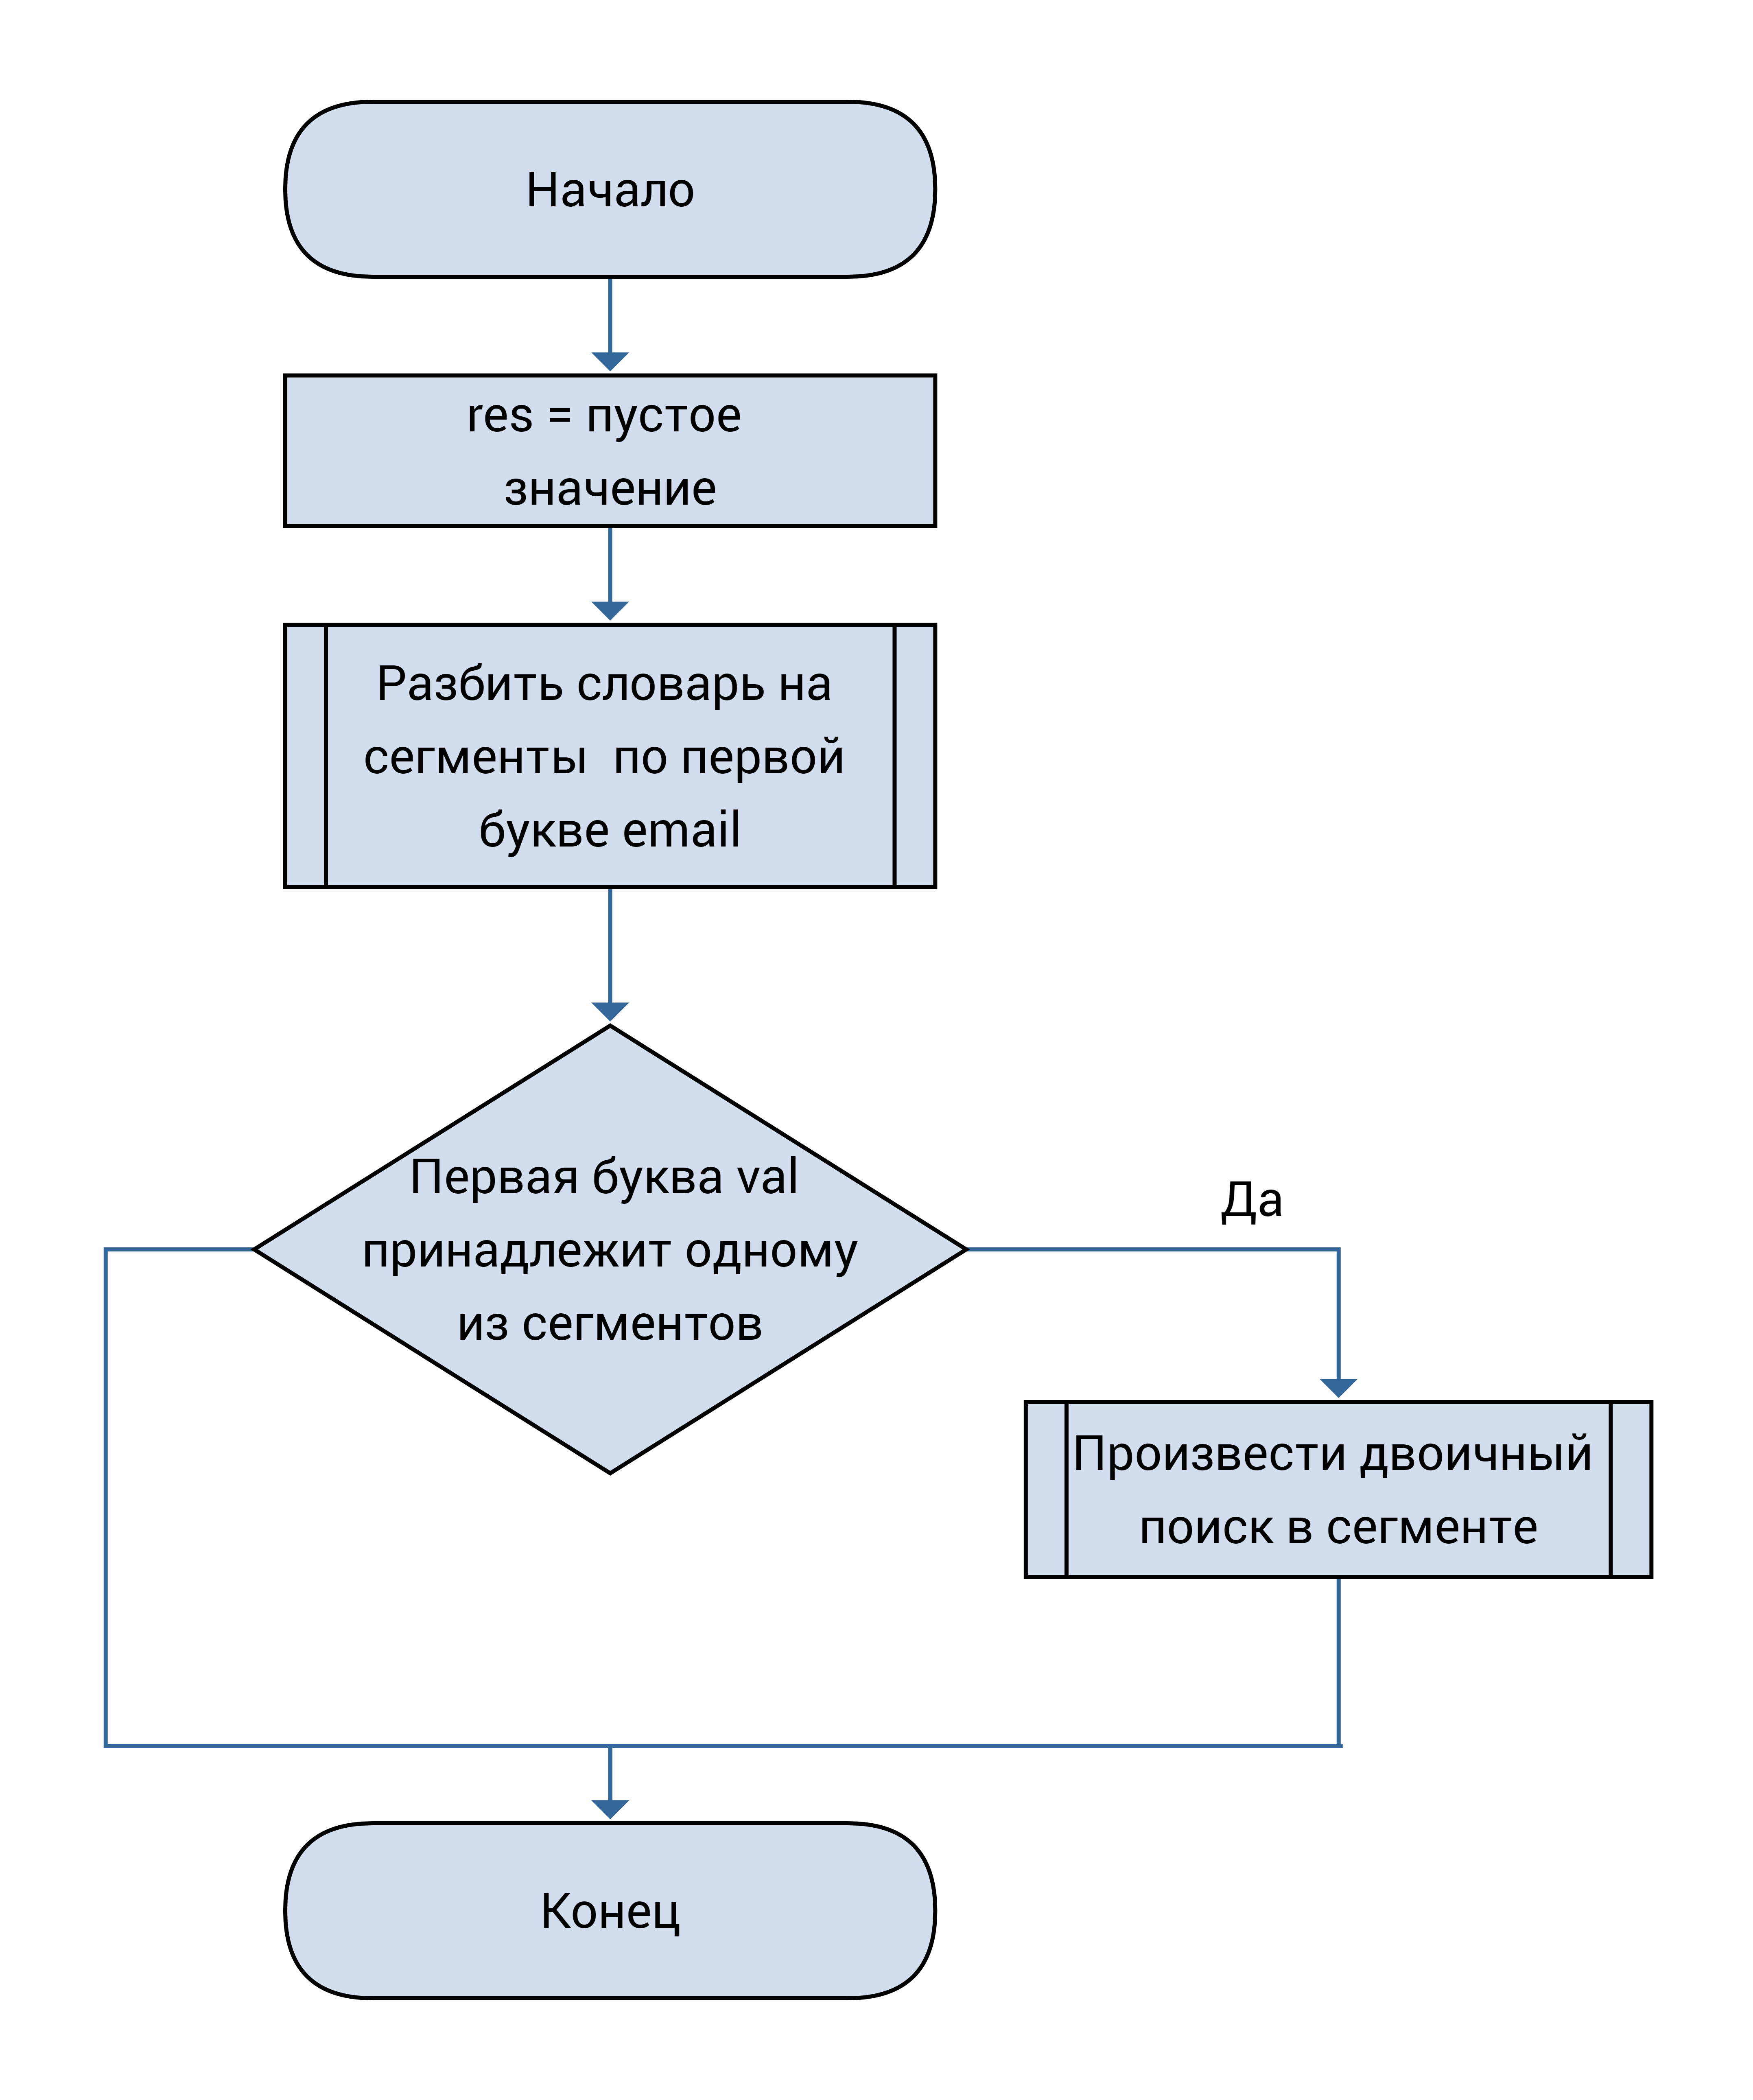
\includegraphics[scale=0.07]{combo}
		\centering\caption{Схема алгоритма комбинированного поиска в словаре.}
	\end{figure}
	\subsection{Вывод}
	\hspace*{5mm} На основе теоретических данных, полученных из аналитического раздела, были построены схемы требуемых алгоритмов. 


\newpage
\section{Технологическая часть}

	\hspace*{5mm} В данном разделе будут рассмотрены требования к программному обеспечению, средства реализации и представлен листинг кода.
	\subsection{Требования к программному обеспечению}
		\begin{enumerate}
		\item на вход подается словарь и значение ключа email;
		\item на выходе - элемент словаря. 
	\end{enumerate}
	\subsection{Средства реализации}
	\hspace*{5mm} В данной работе используется язык программирования Python, за высокую скорость выполнения программ и широкий выбор библиотек.\cite{doc} Проект выполнен в среде разработки Visual Studio Code.
	\clearpage
	\newpage 
	\subsection{Листинг кода}
	На листингах 1, 2, 3 представлена реализация алгоритмов поиска в словаре.
	\definecolor{codegreen}{rgb}{0,0.6,0}
	\definecolor{codegray}{rgb}{0.5,0.5,0.5}
	\definecolor{codepurple}{rgb}{0.58,0,0.82}
	\definecolor{backcolour}{rgb}{0.95,0.95,0.92}

	\lstdefinestyle{mystyle}{
		backgroundcolor=\color{backcolour},   
		commentstyle=\color{codegreen},
		keywordstyle=\color{magenta},
		numberstyle=\tiny\color{codegray},
		stringstyle=\color{codepurple},
		basicstyle=\ttfamily\footnotesize,
		breakatwhitespace=false,         
		breaklines=false,                 
		captionpos=b,                    
		keepspaces=true,                 
		numbers=left,                    
		numbersep=5pt,                  
		showspaces=false,                
		showstringspaces=false,
		showtabs=false,                  
		tabsize=4
	}

	\lstset{style=mystyle}

	\begin{lstlisting}[language=Python, caption = Алгоритм полного перебора]
def full_iteration(emails, val):
	result = None
	if len(emails) == 0:
		return result
	for key, value in emails.items():
		if value == val:
			result = key
	return result
	\end{lstlisting}
\begin{lstlisting}[language=Python, caption = Алгоритм бинарного поиска]
def bin_search(emails, val):
	result = None
	if len(emails) == 0:
		return result
	emails = sort(emails, False)
	mid, low, high = len(emails) // 2, 0, len(emails) - 1
	tmp = tuple(emails.items())
	while tmp[mid][1] != val and low <= high:
		if val > tmp[mid][1]:
			low = mid + 1
		else:
			high = mid - 1
		mid = (low + high) // 2
	if low < high:
		result = tmp[mid][0] 
	return result
\end{lstlisting}
\clearpage
\newpage
\begin{lstlisting}[language=Python, caption = Алгоритм комбинированного поиска]
def combined(emails, val):
	result = None
	if len(emails) == 0:
		return result
	arr = analyse(emails)
	arr = sorted(arr, key = len, reverse = True)
	copy = arr
	for i in range(len(copy)):
		tmp = tuple(copy[i].values())
		if tmp[0][0] == val[0]:
			result = bin_search(arr[i], val) 
	return result 
\end{lstlisting}

	\subsection{Тестирование функций}
	\hspace*{5mm} В таблице 1 приведены функциональные тесты для функций, реализующих алгоритмы поиска в словаре.
	Все тесты прошли успешно.\\
	\begin{table}[h]
		\centering
		\caption{Результаты тестирования.\\}
		\begin{tabular}{ | c | c | c | c |}
			\hline
			Ключ & Пустой словарь & Ожидаемый результат & Результат  \\ \hline
			ann78@hotmail.com & Нет & 700983 &  700983\\ \hline
			ann78@hotmail.com & Да & None &  None\\ \hline
			None & Нет & None &  None\\ \hline
		\end{tabular}
	\end{table}
	
	\subsection{Вывод}
	\hspace*{5mm} В данном разделе была представлена структура ПО и листинги кода программы, а также результаты проведенного тестирования. 
	

\clearpage
\newpage
\section{Исследовательская часть }

	\hspace*{5mm} В данном разделе приведены примеры работы и анализ характеристик разработанного программного обеспечения.
	\subsection{Системные характеристики}
	Характеристики компьютера на котором проводился замер времени сортировки массива:
	\begin{enumerate}
		\item операционная система - Windows 10;
		\item процессор - Intel(R) Core(TM) i7-10510U CPU @1.80GHz 2.30GHz;
		\item оперативная память - 16 ГБ;
		\item количество ядер - 4;
		\item количество логических процессов - 8.
	\end{enumerate}
	\subsection{Пример работы}
	\hspace*{5mm} Демонстрация работы программы приведена на рисунке 4.
	\begin{figure}[h]
		\centering 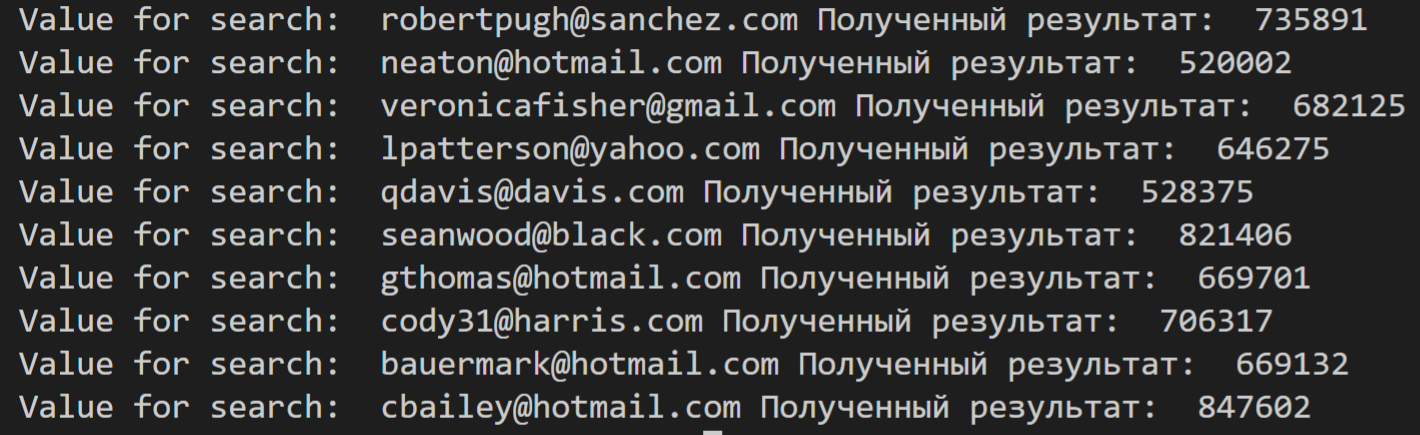
\includegraphics[scale=0.9]{r}
		\centering\caption{Пример работы программы.}
	\end{figure}
	\clearpage
	\newpage
	\subsection{Сравнительный анализ на основе замеров времени работы программы}
	Был проведен замер времени работы каждого алгоритма.
	\\ \hspace*{5mm} В таблице 2 показаны результаты эксперимента, суть которого заключается в анализе зависимости размера словаря от времени поиска при разных алгоритмах.
	\begin{table}[h]
		\centering
		\caption{Результаты эксперимента.\\}
		\begin{tabular}{ | c | c | c | c |}
			\hline
			Размер словаря & Полный перебор & Бинарный поиск & Комбинированный  \\ \hline
			1000 & 0.00547088 & 0.00426798 &  5.42187500\\ \hline
			2000 & 0.00661471 & 0.00486018 &  43.9218750\\ \hline
			3000 & 0.00673328 & 0.00533766 &  293.583333\\ \hline
			4000 & 0.00774536 & 0.00520833 &  845.364583\\ \hline
			5000 & 0.00792178 & 0.01041666 &  2153.65624\\ \hline
		\end{tabular}
	\end{table}
	
	\subsection{Вывод}
	\hspace*{5mm} По проведенному анализу из  эксперимента можно сделать вывод, что лучшее время поиска в словаре получается методом полного перебора, а худшее время - комбинированным способом. Комбинированный алгоритм показал такое время за счет анализа и сортировки значений в словаре. Так как во входном словаре данные могут быть уже отсортированы в обратном порядке, соответственно из-за этого получается такое плохое время. Бинарный алгоритм показал близкий результат с алгоритмом полного перебора. Но если оптимизивать сортировку в бинарном поиске и на вход дать уже отсортированный словарь, то он показал наилучшее время. 
	\clearpage
	\newpage
	\section*{Заключение}
	\addcontentsline{toc}{section}{Заключение}
	\hspace*{5mm} В ходе выполнения работы была достигнута цель выполнены все поставленные задачи:
	\begin{enumerate}
		\item рассмотреть и изучить алгоритмы полного перебора, двоичного поиска и эффективного поиска по словарю;
		\item сравнить временные характеристики каждого из рассмотренных алгоритмов;
		\item на основании проделанной работы сделать выводы.
	\end{enumerate}
	\hspace*{5mm} Если исключить время сортировки из итогового времени, то алгоритмы двоичного поиска и частотного анализа должны показать похожие результаты. А за счет проведенного анализа, комбинированный метод показал бы наилучший результат.    
\clearpage
\newpage

\printbibliography
\addcontentsline{toc}{section}{Список литературы}

\end{document}